% =========================================================================== %

\begin{frame}[t,plain]
\titlepage
\end{frame}

% =========================================================================== %

\begin{frame}{Script}
%
\begin{itemize}
\item Kapitel 8
	\begin{itemize}
	\item 8.1. Arrays
		\begin{itemize}
		\item 8.1.1. Syntax-Elemente
		\item 8.1.2. Initialisierung
		\item 8.1.3. Pointer-Arithmetik
		\item 8.1.4. Mehrdimensionale Arrays
		\end{itemize}
	\item 8.4. Speicherbedarf von Datenstrukturen ermitteln: \mintinline{c}{sizeof}
	\end{itemize}
\end{itemize}
%
\end{frame}

% =========================================================================== %

\begin{frame}{Listen (\enquote{Arrays})}
%
\begin{columns}[T]
\column{.5\linewidth}
\begin{itemize}
\item Container für mehr als eine Zahl
\item Intern: Reserviere \enquote{Speicherblock}
\item Speichere \emph{Pointer} auf Anfang des Blocks
\item Indices beginnen bei 0
\end{itemize}
%
\begin{codebox}[Syntax -- Deklaration]
\mint{c}{Datentyp Variable[Anzahl];}
\end{codebox}
%
\begin{codebox}[Syntax -- Zugriff]
\mint{c}{Variable[Index] = Ausdruck;}
\end{codebox}
%
\column{.5\linewidth}
\begin{warnbox}
Zugriff auf nicht reservierten Bereich undefiniert!
\end{warnbox}
%
\begin{tcolorbox}[title=Speicherbild]
\begin{tikzpicture}
  [ 
    cell/.style={text width=8mm,
      text height=4mm, draw=black, inner sep=1mm},
    ld/.style={draw=blue,shorten >=2pt,->}
  ]
  \node (c1) at (0,0) [cell] {\scriptsize\ttfamily 99};
  \node (c2) at (1,0) [cell] {\scriptsize\ttfamily 1};
  \node (c3) at (2,0) [cell] {\scriptsize\ttfamily 255};
  \node (c4) at (3,0) [cell] {\scriptsize\ttfamily 0};
  \node (c5) at (4,0) [cell] {\scriptsize\ttfamily 80};
  \node (c6) at (5,0) [cell] {\scriptsize\ttfamily ...};
  
  \node (a1) [below=2mm of c1]            {\tiny 0x27ff};
  \node (a2) [below=2mm of c2, color=red] {\tiny 0x2800};
  \node (a3) [below=2mm of c3]            {\tiny 0x2801};
  \node (a4) [below=2mm of c4]            {\tiny 0x2802};
  \node (a5) [below=2mm of c5]            {\tiny 0x2803};
  \node (a6) [below=2mm of c6]            {\tiny 0x2804};
  
  \node (ptr) [below=8mm of c1] {\scriptsize\ttfamily var};
  \node (vc2) [above=6mm of c1] {\scriptsize\ttfamily var[2]};
  \node (vc0) [above=2mm of c1] {\scriptsize\ttfamily var[0]};
  
  \draw [ld] (ptr.east) .. controls +(0.3,0) .. (a2.south);
  \draw [ld] (vc0.east) .. controls +(0.4,0) .. (c2.north);
  \draw [ld] (vc2.east) .. controls +(2.4,0) .. (c4.north);
\end{tikzpicture}
\end{tcolorbox}
%
\end{columns}
%
\end{frame}

% =========================================================================== %

\begin{frame}[fragile]
%
\tcbset{width=.595\linewidth, on line, box align=top}
%
\begin{codebox}[Beispiel]
\begin{minted}[fontsize=\footnotesize,linenos]{c}
#include <stdio.h>

int main () {
  int i;
  int cubes[14];
  
  for (i = 0; i < 14; i++) {
    cubes[i] = i * i * i;
  }
  
  for (i = 0; i < 14; i++) {
    printf("%2d^3 = %4d\n", i, cubes[i]);
  }
  printf("Adresse: %p\n", (void *) cubes);
}
\end{minted}
\end{codebox}%
%
\tcbset{width=.395\linewidth, on line, box align=top}
%
\begin{cmdbox}[Ausgabe]
\begin{minted}[fontsize=\footnotesize]{text}
 0^3 =    0
 1^3 =    1
 2^3 =    8
 3^3 =   27
 4^3 =   64
 5^3 =  125
 6^3 =  216
 7^3 =  343
 8^3 =  512
 9^3 =  729
10^3 = 1000
11^3 = 1331
12^3 = 1728
13^3 = 2197
Adresse: 0x7fff7caa82e0
\end{minted}
\end{cmdbox}
%
\end{frame}

% =========================================================================== %

\begin{frame}[fragile]
%
\tcbset{width=.595\linewidth, on line, box align=center}
%
\begin{warnbox}[Speicherverletzung, leftupper=6mm]
\begin{minted}[fontsize=\scriptsize,linenos]{c}
#include <stdio.h>

int main () {
  int foobar1[1];
  int foobar2[1];
  
  printf("foobar1 : %p\n", (void *) foobar1);
  printf("foobar2 : %p\n", (void *) foobar2);
  printf("\n");
  
  foobar2[0] = 2;
  printf("foobar2[0]: %d\n", foobar2[0]);

  foobar1[1] = 1;  
  printf("foobar2[0]: %d\n", foobar2[0]);
}
\end{minted}
\end{warnbox}%
%
\tcbset{width=.395\linewidth, on line, box align=center}
%
\begin{cmdbox}[Ausgabe]
\begin{minted}[fontsize=\footnotesize]{text}
foobar1 : 0x7ffc3c3b43f0
foobar2 : 0x7ffc3c3b43f4

foobar2[0]: 2
foobar2[0]: 1
\end{minted}
\end{cmdbox}
%
\end{frame}

% =========================================================================== %

\begin{frame}[fragile]
%
\begin{columns}[T]
\column{.45\linewidth}
\begin{Large}
{Pointer-Arithmetik}
\vspace{6pt}
\end{Large}
%
\begin{itemize}
\item Dereferenzierung:					\tabto{3.1cm} \texttt{*pointer}
\item Zugriff auf bestimmtes Element:	\tabto{3.1cm} \texttt{pointer[index]}
\item Adresse finden:					\tabto{3.1cm} \texttt{\&variable}
\item Addition und Subtraktion definiert
\item Gehe \texttt{index} Schritte weiter.
\item Schrittweite: Automatische Anpassung an Datentypen
\item Selten nötig, aber manchmal wichtig, um andere Codes zu verstehen
\item C++: Konzept Iterator
\end{itemize}
%
\column{.55\linewidth}
\begin{codebox}[Arrayzugriff -- mehrere Syntaxes]
\begin{minted}[fontsize=\scriptsize,linenos]{c}
#include <stdio.h>

int main () {
   int i;
   int array[10];
	
   for (i=0; i<10; i++) {array[i] = 2*i;}
	
   printf("%d\n",   array  [5]);
   printf("%d\n", *(array + 5));

   i = 2;
   printf("%d\n", i[array]);  // cringe
}
\end{minted}
\end{codebox}
%
\begin{hintbox}
\footnotesize Benutzt bei Arrays die Variante \texttt{var[i]}!
\end{hintbox}
\end{columns}
%
\end{frame}

% =========================================================================== %

\begin{frame}[fragile]
%
\begin{columns}[T]
\column{.4\linewidth}
\begin{Large}
{\mintinline{c}{sizeof}}
\vspace{6pt}
\end{Large}
%
\begin{itemize}
\item Speicherbedarf einer Struktur ermitteln
\item Funktioniert mit Datentypen, Variablen und Arrays
\item Speicherbedarf in Bytes
\item Konstanten sparen, Programm flexibler ändern
\end{itemize}
%
\begin{hintbox}[Ausblick: VLA]
\footnotesize
Variante \mintinline{c}{int array[variable]} seit C99 möglich, aber gefährlich.
\end{hintbox}
%
\column{.6\linewidth}
%
\begin{codebox}
\begin{minted}[fontsize=\scriptsize,linenos]{c}
#include <stdio.h>

int main () {
  int cubes[14];
  int i, size = sizeof(cubes) / sizeof(*cubes);
  
  for (i = 0; i < size; i++) {
    cubes[i] = i * i * i;
  }
  
  for (i = 0; i < size; i++) {
    printf("%2d^3 = %4d\n", i, cubes[i]);
  }
  
  printf("'cubes' hat %d Elemente.\n", size);
}
\end{minted}
\end{codebox}
%
\end{columns}
%
\end{frame}

% =========================================================================== %

\begin{frame}{Arrays Initialisieren}
%
\begin{columns}[T]
\column{.45\linewidth}
\begin{itemize}
\item Wertzuweisung bei Erstellen\newline
	Wie bei einfachen Variablen
\item Bei zu wenigen Werten: Automatisch 0
\item Mindestens ein Wert muss angegeben werden, darf 0 sein.
\item Zu viele Werte: Speicherverletzung (Compiler gibt Warnung aus)
\item Größe kann automatisch ermittelt werden
\end{itemize}
%
\column{.55\linewidth}
\begin{codebox}[Syntax]
\footnotesize \mint{c}{Datentyp Variable[Anzahl] = {Werte, ...}}
\footnotesize \mint{c}{Datentyp Variable[] = {Werte, ...}}
\end{codebox}
%
\begin{hintbox}
Benutzt die \texttt{[]}-Syntax und \mintinline{c}{sizeof}, um Speicherverletzung zu vermeiden
\end{hintbox}
%
\end{columns}
%
\end{frame}

% =========================================================================== %

\begin{frame}[fragile]
%
\tcbset{width=.545\linewidth, on line, box align=center}
%
\begin{codebox}
\begin{minted}[fontsize=\footnotesize,linenos]{c}
#include <stdio.h>

int main () {
  int i;
  char digits[] = {
    2, 7, 1, 8, 2, 8, 1, 8, 2, 8, 
    4, 5, 9, 0, 4, 5, 2, 3, 5, 3, 
    6, 0, 2, 8, 7, 4, 7};
  
  printf("Euler's number:\n");
  for (i = 0; i < sizeof(digits); i++) {	
    printf("%1d", digits[i]);
    if (i==0) {printf(".");}
  }
}
\end{minted}
\end{codebox}%
%
\tcbset{width=.445\linewidth, on line, box align=center}
%
\begin{cmdbox}[Ausgabe]
Euler's number:\\
2.71828182845904523536028747
\end{cmdbox}
%
\end{frame}

% =========================================================================== %

\begin{frame}{Mehrdimensionale Arrays}
%
\begin{columns}[T]
\column{.5\linewidth}
\begin{tcolorbox}[title=Vorstellung: Matrix/Tabelle]
\begin{table}
	\newcolumntype{M}{>{$} p{.20\linewidth}<{$}}

\begin{tabularx}
	{\linewidth}
	{|M|M|M|M}
	\toprule
	
	a_{11} & a_{12} & \ldots & a_{1n} \tabcrlf
	a_{21} & a_{22} & \ldots & a_{2n} \tabcrlf
	\ldots & \ldots & \ldots & \ldots \tabcrlf
	a_{m1} & a_{m2} & \ldots & a_{mn} \tabcrlf
	
\end{tabularx}
\end{table}
Objekt mit $m$ Zeilen und $n$ Spalten.
\end{tcolorbox}
%
\column{.5\linewidth}
\begin{tcolorbox}[title=Speicher: Liste von Listen]
\texttt{
A = \{\newline
	\tabto{1,4cm}\{$a_{11}$, $a_{12}$, \ldots, $a_{1n}$\},\newline
	\tabto{1,4cm}\{$a_{21}$, $a_{22}$, \ldots, $a_{2n}$\},\newline
	\tabto{3,0cm}\ldots\newline
	\tabto{1,4cm}\{$a_{m1}$, $a_{m2}$, \ldots, $a_{mn}$\}\newline
\}
}
\end{tcolorbox}
Nach diesem Prinzip auch: Listen von Listen von Listen von ... \newline
$\Rightarrow$ \emph{Tensoren}
\end{columns}
%
\end{frame}

% =========================================================================== %

\begin{frame}{Mehrdimensionale Arrays}
%
\begin{columns}[T]
\column{.3\linewidth}
\begin{itemize}
\item Speicherobjekt mit mehreren Indizes
\item Objekt selbst: Pointer
\item Objekt mit $1 \ldots n-1$ Indizes: Pointer
\item Objekt mit $n$ Indizes: Wert selbst
\end{itemize}
%
\column{.7\linewidth}
\begin{codebox}[Syntax: Deklaration]
\texttt{\footnotesize Datentyp var[Zeilen][Spalten]...[Schichten]}
\end{codebox}
%
\begin{codebox}[Syntax: Zugriff]
\texttt{\footnotesize var[Zeilen][Spalten]...[Schichten] = Ausdruck;}
\end{codebox}
%
\end{columns}
%
\vspace{6pt}
%

%
\end{frame}

% =========================================================================== %

\begin{frame}[fragile]{Mehrdimensionale Arrays Initialisieren}
%
\begin{codebox}
\begin{minted}[fontsize=\scriptsize,linenos]{c}
#include <stdio.h>

int main () {
  int digits[2][2][2]  = {
    {   {1, 2}, {3, 4}   }, 
    {   {5, 6}, {7, 8}   }
  };
  
  printf("digits         : %p\n", (void *) digits);
  printf("digits[0]      : %p\n", (void *) digits[0]);
  printf("digits[1]      : %p\n", (void *) digits[1]);
  printf("digits[0][0]   : %p\n", (void *) digits[0][0]);
  printf("digits[0][1]   : %p\n", (void *) digits[0][1]);
  printf("digits[0][0][0]: %d\n",          digits[0][0][0]);
}
\end{minted}
\end{codebox}
%
\end{frame}

% =========================================================================== %

\begin{frame}{Speicherbild Tabelle}
%
\begin{center}
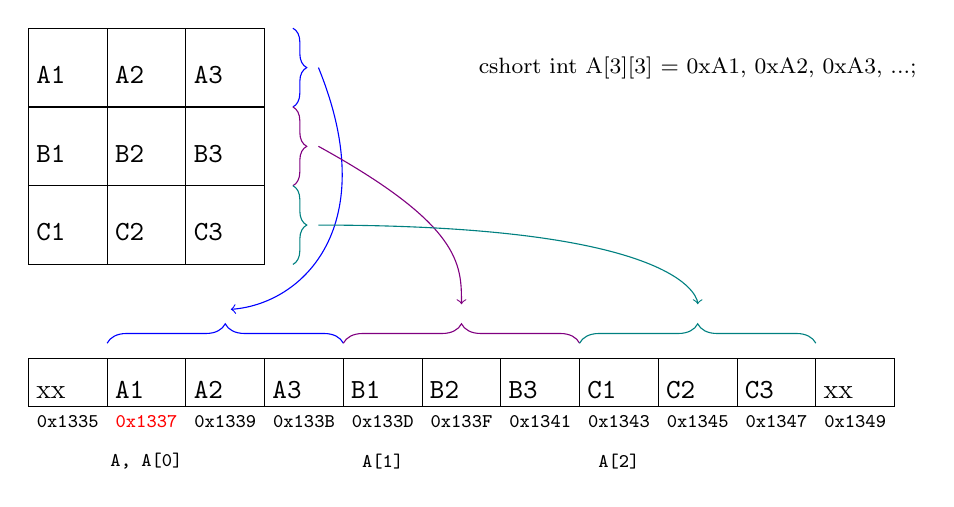
\begin{tikzpicture}
[ 
    cell/.style={text width=8mm,
    text height=4mm, draw=black, inner sep=1mm},
    ld/.style={draw=blue,shorten >=2pt,->},
    flow/.style={draw=black,->,shorten >=2pt}
]  
  \node [draw,minimum height=1cm] (cA1) at (0, 5) [cell] {\texttt{A1}};
  \node [draw,minimum height=1cm] (cA2) at (1, 5) [cell] {\texttt{A2}};
  \node [draw,minimum height=1cm] (cA3) at (2, 5) [cell] {\texttt{A3}};
  
  \node [draw,minimum height=1cm] (cB1) at (0, 4) [cell] {\texttt{B1}};
  \node [draw,minimum height=1cm] (cB2) at (1, 4) [cell] {\texttt{B2}};
  \node [draw,minimum height=1cm] (cB3) at (2, 4) [cell] {\texttt{B3}};
  
  \node [draw,minimum height=1cm] (cC1) at (0, 3) [cell] {\texttt{C1}};
  \node [draw,minimum height=1cm] (cC2) at (1, 3) [cell] {\texttt{C2}};
  \node [draw,minimum height=1cm] (cC3) at (2, 3) [cell] {\texttt{C3}};
  
  \node (m0) at (0, 1) [cell] {xx};
  
  \node (m1) at (1, 1) [cell] {\texttt{A1}};
  \node (m2) at (2, 1) [cell] {\texttt{A2}};
  \node (m3) at (3, 1) [cell] {\texttt{A3}};
  \node (m4) at (4, 1) [cell] {\texttt{B1}};
  \node (m5) at (5, 1) [cell] {\texttt{B2}};
  \node (m6) at (6, 1) [cell] {\texttt{B3}};
  \node (m7) at (7, 1) [cell] {\texttt{C1}};
  \node (m8) at (8, 1) [cell] {\texttt{C2}};
  \node (m9) at (9, 1) [cell] {\texttt{C3}};

  \node (mx) at (10, 1) [cell] {xx};
  
  \draw [decorate, decoration={brace, amplitude=5pt, mirror}, xshift=-4pt, yshift=0pt, blue]
  		(3.0, 4.5) -- (3.0, 5.5) 
  		node [midway, xshift=+0.2cm]
		(lA) {};
  \draw [decorate, decoration={brace, amplitude=5pt, mirror}, xshift=-4pt, yshift=0pt, violet]
  		(3.0, 3.5) -- (3.0, 4.5) 
  		node [midway, xshift=+0.2cm]
		(lB) {};
  \draw [decorate, decoration={brace, amplitude=5pt, mirror}, xshift=-4pt, yshift=0pt, teal]
  		(3.0, 2.5) -- (3.0, 3.5) 
  		node [midway, xshift=+0.2cm]
		(lC) {};
  
  \draw [decorate, decoration={brace,amplitude=7pt}, xshift=-0pt, yshift=0pt, blue]
  		(0.5, 1.5) -- (3.5, 1.5) node [black, midway, yshift=+0.3cm] 
		(mA) {};
  \draw [decorate, decoration={brace,amplitude=7pt}, xshift=-0pt, yshift=0pt, violet]
  		(3.5, 1.5) -- (6.5, 1.5) node [black, midway, yshift=+0.3cm] 
		(mB) {};
  \draw [decorate, decoration={brace,amplitude=7pt}, xshift=-0pt, yshift=0pt, teal]
  		(6.5, 1.5) -- (9.5, 1.5) node [black, midway, yshift=+0.3cm] 
		(mC) {};
  
  \draw[flow, blue]   (lA.east) .. controls (4, 3) and (3, 2.0) .. (mA.north);
  \draw[flow, violet] (lB.east) .. controls (5, 3) and (5, 2.5) .. (mB.north);
  \draw[flow, teal]   (lC.east) .. controls (8, 3) and (8, 2.0) .. (mC.north);
  
  \node (a0) at (0, 0.5)       {\scriptsize\texttt{0x1335}};
  
  \node (a1) at (1, 0.5) [red] {\scriptsize\texttt{0x1337}};
  	\node (x0) at (1, 0)       {\scriptsize\texttt{A, A[0]}};
  \node (a2) at (2, 0.5)       {\scriptsize\texttt{0x1339}};
  \node (a3) at (3, 0.5)       {\scriptsize\texttt{0x133B}};
  \node (a4) at (4, 0.5)       {\scriptsize\texttt{0x133D}};
  	\node (x1) at (4, 0)       {\scriptsize\texttt{A[1]}};
  \node (a5) at (5, 0.5)       {\scriptsize\texttt{0x133F}};
  \node (a6) at (6, 0.5)       {\scriptsize\texttt{0x1341}};
  \node (a7) at (7, 0.5)       {\scriptsize\texttt{0x1343}};
  	\node (x2) at (7, 0)       {\scriptsize\texttt{A[2]}};
  \node (a8) at (8, 0.5)       {\scriptsize\texttt{0x1345}};
  \node (a9) at (9, 0.5)       {\scriptsize\texttt{0x1347}};
  
  \node (a0) at (10, 0.5)      {\scriptsize\texttt{0x1349}};
  
  \node (code) at (8, 5) {\footnotesize\mintinline{c}{short int A[3][3] = {{0xA1, 0xA2, 0xA3}, ...};}};
\end{tikzpicture}
\end{center}
%
\end{frame}

% =========================================================================== %

\begin{frame}[fragile]{Mehrdimensionale Arrays}
%
\tcbset{width=.495\linewidth, height=4.9cm, on line}
%
\begin{warnbox}[Auf Reihenfolge der Indizes achten]
\footnotesize
Mehrdimensionale automatische Arrays werden auf eindimensionale Listen \enquote{geplättet}. Der Index der geplätteten Liste berechnet sich (bei 2 Dimensionen) nach
\begin{center}
\texttt{\scriptsize Index = Zeile * Breite + Spalte}
\end{center}
Vertauschte Indizes ergeben daher nicht nur Zugriffe auf falsche Zellen, sondern ggf. auch auf nicht reservierte Speicherbereiche!
\end{warnbox}
%
%\column{.43\linewidth}
\begin{codebox}
\begin{minted}[fontsize=\scriptsize,linenos]{c}
#include <stdio.h>

int main () {
  int tab[3][4]  = {
    { 1,  2,  3,  4},
    { 5,  6,  7,  8},
    { 9, 10, 11, 12}
  };
  
  printf("%d\n", tab[2][3]);  // ok
  printf("%d\n", tab[3][2]);  // !!
}
\end{minted}
\end{codebox}
%
\tcbset{width=\linewidth, height=1.7cm, on line}
%
\begin{cmdbox}[Ausgabe]
\footnotesize
12\\
1235439616
\end{cmdbox}
%
\end{frame}

% =========================================================================== %

\begin{frame}{Script}
%
\begin{itemize}
\item Kapitel 8
	\begin{itemize}
	\item 8.3. C-Strings
		\begin{itemize}
		\item 8.3.1. spezielle Syntax-Elemente
		\item 8.3.2. User-Eingaben
		\end{itemize}
	\end{itemize}
\end{itemize}
%
\end{frame}

% =========================================================================== %

\begin{frame}[fragile]
%
\begin{columns}[T]
\column{.405\linewidth}
\begin{Large}
{Zeichenketten -- Strings}
\vspace{6pt}
\end{Large}
\begin{itemize}
\item \enquote{Liste von Zeichen}: \mintinline{c}{char}-Arrays
\item Zahlen, die über ASCII-Tabelle \enquote{in Schriftzeichen übersetzt} werden
\item \emph{Nullterminiert}
\item Tools in \texttt{string.h} definiert
\item Syntaxelement 1: \texttt{'}einfache Anfürungszeichen\texttt{'}: ASCII-Code zum Schriftzeichen
\end{itemize}
%
\column{.645\linewidth}
\begin{codebox}[Beispiel: Wertzuweisung Strings (1)]
\begin{minted}[fontsize=\footnotesize,linenos]{c}
#include <stdio.h>

int main () {
  char string[] = {
    'D', 'u', 'n', 'e', ' ', 'b', 'y', ' ', 
    'F', 'a', 'n', 'k', ' ', 
    'H', 'e', 'r', 'b', 'e', 'r', 't', 0};
}
\end{minted}
\end{codebox}
%
\begin{warnbox}
Stellt genug Speicherplatz für Strings zur Verfügung!\newline
Denkt auch an das Null-Zeichen!
\end{warnbox}
%
\end{columns}
%
\end{frame}

% =========================================================================== %\\

\begin{frame}[fragile]
%
\begin{columns}[T]
\column{.405\linewidth}
\begin{Large}
{Zeichenketten -- Strings}
\vspace{6pt}
\end{Large}
%
\begin{itemize}
\item Syntaxelement 2: Kompakte Fassung mit \texttt{''}doppelten Anführungszeichen\texttt{''}
\item Null-Zeichen wird automatisch angehängt
\item Beschreibt eigentlich einen Pointer auf die Code-Stelle, an der der Text steht
\item Bei der Deklaration aber direkte Zuweisung möglich.
\end{itemize}
%
\column{.645\linewidth}
\begin{codebox}[Beispiel: Wertzuweisung Strings (2)]
\begin{minted}[fontsize=\footnotesize,linenos]{c}
#include <stdio.h>

int main () {
  char string[] = "Dune by Frank Herbert";
}
\end{minted}
\end{codebox}
%
\begin{warnbox}
Diese Art der Zuweisung ist nur bei der Deklaration möglich.
\end{warnbox}
%
\end{columns}
%
\end{frame}

% =========================================================================== %

\begin{frame}[fragile]{Strings als Usereingaben}
%
\begin{codebox}
\begin{minted}[fontsize=\scriptsize,linenos]{c}
#include <stdio.h>

int main () {
   char s[11];

   printf("Bitte geben Sie bis zu 10 Zeichen ein!\n");
   scanf("%10s", s);  // KEIN &s!

   printf("\nSie haben eingebeben:\n %s\n", s);
}
\end{minted}
\end{codebox}
%
\begin{hintbox}
Usereingabe begrenzen mit \texttt{\%Ns}. N: Zahl der maximal einzugebenden Zeichen
\end{hintbox}
%
\end{frame}

% =========================================================================== %

\begin{frame}[fragile]{Beispiel -- Zugriff auf String-Elemente}
%
\begin{columns}[T]
\column{.6\linewidth}
\begin{codebox}
\begin{minted}[fontsize=\scriptsize,linenos]{c}
#include <stdio.h>

int main () {
   char s[] = "lower case";
   int i;

   printf("Original Text:\n%s\n", s);
   
   for (i=0; i<sizeof(s); i++) {
      s[i] -= ' ';
   }

   printf("Converted to upper case:\n%s\n", s);
}
\end{minted}
\end{codebox}
%
\column{.4\linewidth}
\begin{cmdbox}[Ausgabe]
\ttfamily \footnotesize
Original Text:\newline
lower case\newline
Converted to upper case:\newline
LOWER
\end{cmdbox}
%
\begin{warnbox}
''Double Quotes'' für Strings

'Simple Quotes' für \emph{einzelne} chars
\end{warnbox}
\end{columns}
%
\end{frame}

% =========================================================================== %

\begin{frame}{Script}
%
\begin{itemize}
\item Kapitel 15
	\begin{itemize}
	\item 15.2. Zufallszahlen
	\end{itemize}
\end{itemize}
%
\end{frame}

% =========================================================================== %

\begin{frame}[fragile]{Zufallszahlen}
%
\begin{columns}[T]
\column{.5\linewidth}
\begin{itemize}
\item Pseudo-Zufallszahlen: $x_i = f(x_{i-1})$
\item Startwert legt alle weiteren fest
\item Setze Startwert auf Uhrzeit\newline
	$\Rightarrow$ zufällige Reihe
\item Zufalls-Funktionen definiert in \texttt{stdlib.h}
\item Zeit-Funktionen definiert in \texttt{time.h}
\item int-Werte zwischen 0 und \texttt{RAND\_MAX}
\item Header: \mintinline{c}{#include <stdlib.h>}, \mintinline{c}{#include <time.h>}
\item[$\Rightarrow$] \url{http://de.cppreference.com/w/c/numeric/random/rand}
\end{itemize}
%
%
\column{.5\linewidth}
\begin{codebox}[Syntax: Startwert setzen]
\mint{c}{srand(init_value);}
\end{codebox}
%
\begin{codebox}[Syntax: Sekunden seit Mitternacht]
\mint{c}{seconds = time(NULL);}
\end{codebox}
%
\begin{codebox}[Syntax: Zufallszahl abrufen]
\mint{c}{number = rand();}
\end{codebox}
\end{columns}
%
\end{frame}

% =========================================================================== %

\begin{frame}[fragile]{Beispiel}
%
\begin{codebox}
\begin{minted}[fontsize=\scriptsize,linenos]{c}
#include <stdio.h>
#include <stdlib.h>
#include <time.h>

int main () {
  int lower = 0, upper = 5;
  
  srand(time(NULL));
  
  printf("Random number between %d and %d:\n", lower, upper);
  printf("%d\n",    lower   +   rand()   %   (upper - lower + 1)   );
  
  printf("Double value between 0 and 1:\n");
  printf("%lf\n", rand() / RAND_MAX);
}
\end{minted}
\end{codebox}
%
\end{frame}